\chapter{Quadratic Form}

\section{Mathematical and Geometric Ideas of Quadratic Form}
\subsection{Definition of Quadratic Form}

Symmetric matrices often see their appearance in the areas of Geometry, Statistics, Physics, and more. One of their usages are the creation of the quadratic form. The word quadratic is commonly associated to quadratic equations commonly in the form of $y = ax^2 + bx + c$. Quadratic forms are the generalization of quadratic equations. If there are multiple variables $x_1, x_2, x_3, \cdots, ...$, then possible quadratic forms are made up of the usual quadratic terms $x_1^2, x_2^2, x_3^2, \cdots$, as well as the cross product terms $x_px_q$, $p \neq q$. The usual quadratic terms are just another kind of cross product terms when $p = q$.
\begin{defn}
\label{quadform}
Quadratic forms of multiple variables $x_1, x_2, x_3, \cdots, ...$ has a structure of
\begin{align*}
\sum_{p=1}^{n}\sum_{q=1}^{n} \alpha_{pq} x_px_q
\end{align*}
\end{defn}
For examples, in two variables situation, $x^2 + 3xy + y^2$, $3x^2 - 4xy$ are quadratic forms, while $x^2 + y$, $x + xy + xy^2$ are not. Notice that $x_px_q$ and $x_qx_p$ are the same term, and we will replace $\alpha_{pq}$ or $\alpha_{qp}$ by $\frac{1}{2}(\alpha_{pq} + \alpha_{qp})$ as a single coefficient for both of them. We can always express any quadratic form using symmetric matrix. 
\begin{proper}
For multiple variables expressed in a vector $\vec{x} = (x_1, x_2, x_3, \cdots, ...)^T$, all quadratic terms can be expressed as
\begin{align*}
\vec{x}^TA\vec{x}
\end{align*}
where $A$ is symmetric. Using the definition above, $A$ will has the form of
\begin{align*}
\left[\begin{array}{@{}cccc@{}}
\alpha_{11} & \frac{1}{2}(\alpha_{12} + \alpha_{21}) & \frac{1}{2}(\alpha_{13} + \alpha_{31}) & \cdots \\
\frac{1}{2}(\alpha_{12} + \alpha_{21}) & \alpha_{22} & \frac{1}{2}(\alpha_{23} + \alpha_{32}) &  \\
\frac{1}{2}(\alpha_{13} + \alpha_{31}) & \frac{1}{2}(\alpha_{23} + \alpha_{32}) & \alpha_{33} &  \\
\vdots & & & \ddots
\end{array}\right]
\end{align*}
\end{proper}
For instance, the quadratic form $x^2 - 2xy + 3y^2$ can be rewritten as
\begin{align*}
\begin{bmatrix}
x & y
\end{bmatrix}
\begin{bmatrix}
1 & -1 \\
-1 & 3
\end{bmatrix}
\begin{bmatrix}
x \\
y
\end{bmatrix}
\end{align*}
Short Exercise: Verify the quadratic form by expanding it.

\subsection{Conic Sections}
\label{Conic}
Conic Sections are the name given to a collection of three two-dimensional geometric objects, ellipses/circles, parabola and hyperbola. The name originates from the fact that they can be created by intersecting a plane with a double cone.
\begin{center}
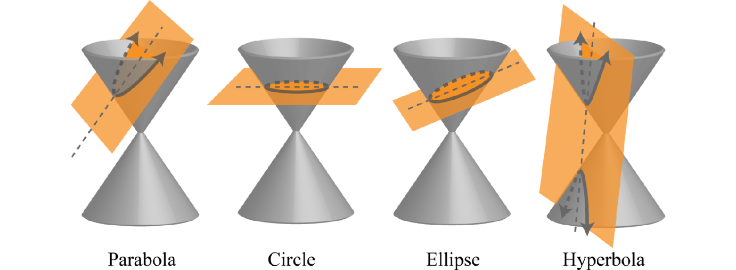
\includegraphics[scale = 0.5]{ConicSection.png}\\
(Taken from Geogebra)
\end{center}
Except parabola, others can be expressed in terms of quadratic forms. What distinguishes them is the discriminant of the quadratic equation.
\begin{proper}
Ellipses, circles, and hyperbola centered at the origin have the form of
\begin{align*}
ax^2 + bxy + cy^2 = h
\end{align*}
where $a$, $b$, $c$ and $h$ are all constants. They can be classified by the discriminant $\Delta = b^2 - 4ac$. The discriminant is positive if the graph is a hyperbola. It is negative if the graph is an ellipse (additionally $b = 0$ and $a = c$ with a circle). However, there are chances that there are no real curves regardless of the value of discriminant. They can be written as $\vec{x}^TA\vec{x} = h$, where
\begin{align*}
A &= 
\begin{bmatrix}
a & \frac{1}{2}b \\
\frac{1}{2}b & c
\end{bmatrix}
\end{align*}
Notice that the determinant $\det(A)$ is $-\frac{1}{4}$ of the discriminant.
\end{proper}
The statement above does not mention what happens when the discriminant is zero. In fact it is due to the removal of linear terms in the quadratic forms. Quadratic equations, in the most general sense, have the form of $ax^2 + bxy + cy^2 + mx + ny = h$, with $m$ and $n$ are constants as well. A zero discriminant actually represents parabola, but the lack of linear terms in quadratic terms reduces the parabola to straight lines. Of course we can include the linear terms to encompass the parabola as well, but to make our discussion below simpler, we will stick to the quadratic form expression and only talk about the central conics.\\
Short Exercise: Identify the types of curve generated by $x^2 - xy + 2y^2 = 3$ and $x^2 + xy - y^2 = 1$.
\begin{center}
\begin{tikzpicture}
\draw[thick, ->] (-3,0) -- (3,0) node[right]{$x$};
\draw[thick, ->] (0,-3) -- (0,3) node[above]{$y$};
\draw[Green,rotate=30] plot[domain=-0.8:1] ({2*cosh(\x)},{1.5*sinh(\x)});
\draw[Green,rotate=30] plot[domain=-1:0.8] ({-2*cosh(\x)},{1.5*sinh(\x)});
\draw[red,rotate=30] plot[domain=-3:3] ({\x},{0});
\draw[blue,rotate=-60] plot[domain=-3:3] ({\x},{0});
\end{tikzpicture}
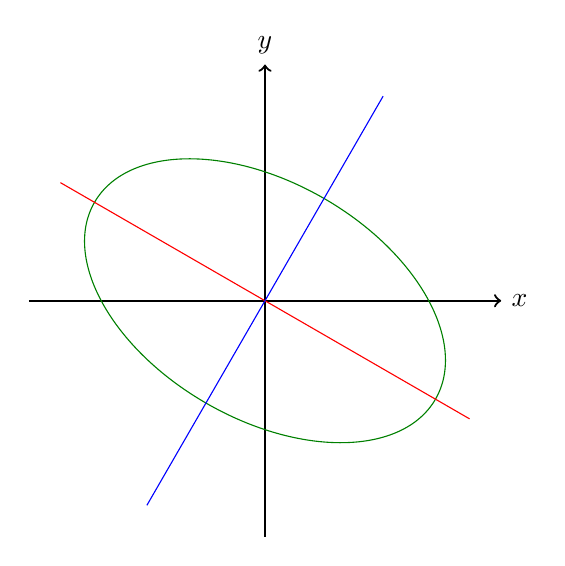
\begin{tikzpicture}
\draw[thick, ->] (-3,0) -- (3,0) node[right]{$x$};
\draw[thick, ->] (0,-3) -- (0,3) node[above]{$y$};
\draw[Green, rotate=-30] (0,0) ellipse (2.5 and 1.5);
\draw[red,rotate=-30] plot[domain=-3:3] ({\x},{0});
\draw[blue,rotate=60] plot[domain=-3:3] ({\x},{0});
\end{tikzpicture} \\
Left: A hyperbola ($\frac{11}{144}x^2 + \frac{25}{24\sqrt{2}}xy - \frac{13}{48}y^2 = 1$), Right: An ellipse ($\frac{52}{225}x^2 + \frac{32}{75\sqrt{3}}xy + \frac{28}{75}y^2 = 1$). Both of them are rotated in the sense that their major axis (red) and minor axis (blue) are not aligned and made a angle of 30 degrees with the $x$ and $y$ axes. Major axis always passes through the vertices, with the minor axis perpendicular to it.
\end{center}

The last properties actually has another interpretation in terms of matrix. But before that we need to introduce some new terminologies.
\begin{defn}
For any symmetric matrix $A$, the quadratic form $\vec{x}^T A\vec{x}$ is called
\begin{enumerate}[label=(\alph*)]
\item positive definite, if for any $\vec{x} \neq \vec{0}$, $\vec{x}^T A\vec{x} > 0$ (positive semi-definite if $\vec{x}^T A\vec{x} \geq 0$), 
\item negative definite, if for any $\vec{x} \neq \vec{0}$, $\vec{x}^T A\vec{x} < 0$ (negative semi-definite if $\vec{x}^T A\vec{x} \leq 0$), 
\item indefinite if $\vec{x}^T A\vec{x}$ can take both positive and negative values,
\end{enumerate}
\end{defn}
\begin{thm}
The quadratic form $\vec{x}^T A\vec{x}$ is
\begin{enumerate}[label=(\alph*)]
\item positive definite, if and only if all eigenvalues of $A$ are positive (positive semi-definite if and only if all eigenvalues of $A$ are non-negative), 
\item negative definite, if and only if all eigenvalues of $A$ are negative (negative semi-definite if and only if all eigenvalues of $A$ are non-positive), 
\item indefinite when there are both positive and negative eigenvalues for $A$.
\end{enumerate}
\end{thm}
Now we are ready to extend our results and see what the quadratic equation $\vec{x}^TA\vec{x} = h$ can give.
\begin{thm}
Given $\vec{x}^TA\vec{x} = h$, where $h$ is chosen to be $1$ for scaling, then it represents
\begin{enumerate}[label=(\alph*)]
\item an ellipse if $A$ is positive definite,
\item a hyperbola if $A$ is indefinite,
\item no real graph if $A$ is negative definite.
\end{enumerate}
\end{thm}
For example, the quadratic equation $\vec{x}^TA\vec{x} = 1$, where
\begin{align*}
A &=
\begin{bmatrix}
1 & -2 \\
-2 & 3
\end{bmatrix}
\end{align*}
is equivalent to $x^2 - 4xy + 3y^2 = 1$. $A$ has an eigenvalue of $\lambda = 2 \pm \sqrt{5}$. As $\lambda_+ = 2 + \sqrt{5} > 0$ and $\lambda_- = 2 - \sqrt{5} < 0$, $A$ is indefinite and the curves are a pair of hyperbola.\\
\\
The figure in the last page shows that hyperbola and ellipses can be rotated. The effect on the resulted quadratic equation is to produce cross-product terms ($xy$ in two-dimensional cases), which can be eliminated by a rotation to restore the curves so that the major and minor axes are oriented along the $x$ and $y$ axes. If the graphs start with tilted by an angle of $\theta$, we can make a rotation by the same angle $\theta$ but in an opposite sense to recover the standard position. It is equivalent to rotate the coordinate system by an angle of $\theta$ in the same sense of the initial tilting. Section \ref{orthogeometricsub} can be referenced.

\begin{exmp}
Rotate the quadratic equation $x^2 - xy + y^2 = 1$ so that the major axis lies along the $x$-axis. \\
\\
First, we cast the equation into quadratic form $\vec{x}^T A\vec{x}$, with
\begin{align*}
A &=
\begin{bmatrix}
1 & -\frac{1}{2} \\
-\frac{1}{2} & 1
\end{bmatrix}
\end{align*}
We first find the eigenvalues of $A$, the characteristic equation is
\begin{align*}
(1-\lambda)^2 - (-\frac{1}{2})^2 &= 0 \\
\lambda^2 - 2\lambda + \frac{3}{4} &= 0 \\
\lambda &= \frac{1}{2} \text{ or } \frac{3}{2}
\end{align*}
So by the theorem above, $A$ is positive definite and it is an ellipse. We will see very soon the smaller eigenvalue actually corresponds to the major axis. Now we consider an orthogonal matrix $P$ to perform a rotation on the coordinate system, with the old coordinates related to the new coordinates by $\vec{x} = P\vec{x'}$. So the quadratic form is transformed to
\begin{align*}
(P\vec{x'})^T A (P\vec{x'}) &= \vec{x'}^T (P^T AP) \vec{x'}
\end{align*}
We immediately identify $P^T AP$ as a rotation of the coordinate system for the matrix $A$, as noted by the remark at the end of section \ref{orthogonaldiagreal}. The same section tells us that we can deal with the cross product terms by orthogonal diagonalization, which removes the off-diagonal entries in $A$. The normalized eigenvectors are
\begin{align*}
&\vec{v_\lambda} = \begin{bmatrix}
\frac{1}{\sqrt{2}} \\
\frac{1}{\sqrt{2}}
\end{bmatrix}
\text{ for } \lambda = \frac{1}{2}
& \begin{bmatrix}
-\frac{1}{\sqrt{2}} \\
\frac{1}{\sqrt{2}}
\end{bmatrix}
\text{ for } \lambda = \frac{3}{2}
\end{align*}
Hence we can set 
\begin{align*}
P =
\begin{bmatrix}
\frac{1}{\sqrt{2}} & -\frac{1}{\sqrt{2}} \\
\frac{1}{\sqrt{2}} & \frac{1}{\sqrt{2}}
\end{bmatrix}
\end{align*}
So that
\begin{align*}
P^T AP = 
\begin{bmatrix}
\frac{1}{\sqrt{2}} & \frac{1}{\sqrt{2}} \\
-\frac{1}{\sqrt{2}} & \frac{1}{\sqrt{2}}
\end{bmatrix}
\begin{bmatrix}
1 & -\frac{1}{2} \\
-\frac{1}{2} & 1
\end{bmatrix}
\begin{bmatrix}
\frac{1}{\sqrt{2}} & -\frac{1}{\sqrt{2}} \\
\frac{1}{\sqrt{2}} & \frac{1}{\sqrt{2}}
\end{bmatrix}
=
\begin{bmatrix}
\frac{1}{2} & 0\\
0 & \frac{3}{2}
\end{bmatrix}
= D
\end{align*}
The smaller eigenvalue is located at the first row/column, meaning now the major axis matches the new $x$-axis. The new equation is seen to be $\vec{x'}^T D\vec{x}$, or $\frac{1}{2}(x')^2 + \frac{3}{2}(y')^2 = 1$. Below are the diagrams before and after the rotation.

\begin{center}
\begin{tikzpicture}
\draw[thick, ->] (-3,0) -- (3,0) node[right](vecu){$x$};
\draw[thick, ->] (0,-3) -- (0,3) node[above]{$y$};
\draw[Green, thick, rotate=45] (0,0) ellipse ({1.2*sqrt(2)} and {1.2*sqrt(2/3)});
\draw[red, ->] (0,0) -- (2,2) node[above right](vecv){$x'$, Major axis, $\lambda = 1/2$};
\draw[blue, ->] (0,0) -- (-1,1) node[above left]{$y'$, Minor axis, $\lambda = 3/2$};
\node[Green] at (2,-2) {$x^2 - xy + y^2 = 1$};
\pic[draw, ->, "$45^\circ$", angle eccentricity=1.75] {angle = vecu--0--vecv};
\end{tikzpicture}
(Before rotation) \\
\begin{tikzpicture}
\draw[red, thick, ->] (-3,0) -- (3,0) node[right](vecu){$x'$};
\draw[blue, thick, ->] (0,-3) -- (0,3) node[above]{$y'$};
\draw[Green, thick, rotate=0] (0,0) ellipse ({1.2*sqrt(2)} and {1.2*sqrt(2/3)});
\node[Green] at (2,-2) {$\frac{1}{2}(x')^2 + \frac{3}{2}(y')^2 = 1$};
\end{tikzpicture} 
(After rotation)
\end{center}
The degree of tilting can be found to be exactly $\pi/4 = 45^{\circ}$, by comparing the general two-dimensional rotation matrix
\begin{align*}
\begin{bmatrix}
\cos \theta & -\sin \theta \\
\sin \theta & \cos \theta
\end{bmatrix}
\end{align*}
against $P$. $\cos \theta = \frac{1}{\sqrt{2}}$ and $\sin \theta = \frac{1}{\sqrt{2}}$ implies that $\tan \theta = 1$, and $\theta = \pi/4$. The possibility of eliminating the cross-product terms in quadratic forms is formally known as the Principal Axes Theorem.
\end{exmp}
\begin{thm}
For a quadratic form $\vec{x}^TA\vec{x}$, where $A$ is symmetric, we can always make an orthogonal change of variable $\vec{x'} = P^T\vec{x}$ or $\vec{x} = P\vec{x'}$ such that it turns into $\vec{x'}^TD\vec{x'} = \lambda_1 x_1'^2 + \lambda_2 x_2'^2 + \cdots$ which contains no cross-product terms. $P$ is formed by the set of orthonormal column eigenvectors of $A$ and $D$ is a diagonal matrix with entries being the eigenvalues of $A$.
\end{thm}
In general, for a two-dimensional quadratic form
\begin{align*}
\begin{bmatrix}
a & b \\
b & c
\end{bmatrix}
\end{align*}
It can undergo a rotation of the coordinate system by an angle $\theta$ such that
\begin{align*}
\begin{bmatrix}
\cos \theta & \sin \theta \\
-\sin \theta & \cos \theta
\end{bmatrix}
\begin{bmatrix}
a & b \\
b & c
\end{bmatrix}
\begin{bmatrix}
\cos \theta & -\sin \theta \\
\sin \theta & \cos \theta
\end{bmatrix}
=
\begin{bmatrix}
* & 0\\
0 & *
\end{bmatrix}
\end{align*}
the off-diagonal elements become zero. The required $\theta$ is found by  expanding the left hand side and equating both sides, which gives
\begin{align*}
-\sin \theta (a \cos\theta + b\sin \theta) + \cos\theta (b \cos \theta + c\sin \theta) &= 0 \\
\frac{c-a}{2} \sin (2\theta) + b\cos(2\theta) &= 0 \\
\cot(2\theta) &= \frac{a-c}{2b}
\end{align*}
where we apply the familiar double angle formulas.

\section{Statistics with Quadratic Form}
\subsection{Variance}
\label{variancesec}
\subsubsection{Single Distribution}
One important measure in the world of Statistics is the variance of a distribution, or a time-series. Variance can be viewed as the spread of a distribution. Below is the definition of variance for a distribution made up by one single variable.
\begin{defn}
\label{variance}
For a distribution $X$, with $n$ data $x_1, x_2, x_3, \cdots, x_n$, its population variance is
\begin{align*}
\sigma^2 = \text{Var}(X) &= \frac{1}{n} ((x_1 - \mu)^2 + (x_2 - \mu)^2 + (x_3 - \mu)^2 + \cdots + (x_n - \mu)^2) \\
&= \frac{1}{n} \sum_{k=1}^n (x_k - \mu)^2
\end{align*}
where $\mu$ is the mean, or expected value of $X$, and is computed by
\begin{align*}
\mu = E(X) = \frac{1}{n} (x_1 + x_2 + x_3 + \cdots + x_n)
\end{align*}
\end{defn}
A simpler formula for computing the population variance is
\begin{align*}
\sigma^2 = E(X^2) - (E(X))^2 = E(X^2) - \mu^2
\end{align*}
For a finite sample, we may also want to use the sample variance $s^2$, which is the population variance multiplied by a factor of $\frac{n}{n-1}$. \\
As an example, given a dataset $X$, with $5$ data $\vec{x} = (1, 3, 6, 9, 11)^T$, then the mean is
\begin{align*}
\mu = \frac{1}{5}(1 + 3 + 6 + 9 + 11) = 6
\end{align*}
and the population variance is
\begin{align*}
\sigma^2 = \frac{1}{5}((1-6)^2 + (3-6)^2 + (6-6)^2 + (9-6)^2 + (11-6)^2) = 13.6
\end{align*}
We can also use the short-cut formula.
\begin{align*}
\sigma^2 &= E(X^2) - \mu^2 \\
&= \frac{1}{5} (1^2 + 3^2 + 6^2 + 9^2 + 11^2) - 6^2 \\
&= 49.6 - 36 \\
&= 13.6
\end{align*}
Short Exercise: Find the sample variance of $X$.\\
\\
The variance formula in Definition \ref{variance} can be written in quadratic form as follows.
\begin{proper}
Given a distribution $X$, with $n$ data $\vec{x} = (x_1, x_2, x_3, \cdots, x_n)^T$, and a mean of $\mu$, the population variance can be written as
\begin{align*}
\frac{1}{n} (\vec{x'}\cdot\vec{x'}) = \frac{1}{n} \textbf{x}'^T \textbf{x}'
\end{align*}
where $\textbf{x}' = \vec{x'} = \vec{x} - \mu$ is the centered distribution with the mean $\mu$ removed. It can also be expressed as the quadratic form $\vec{x'}^T B'\vec{x'}$, where
\begin{align*}
B' &=
\begin{bmatrix}
\frac{1}{n} & 0 & 0 & \cdots \\
0 & \frac{1}{n} & 0 & \\
0 & 0 & \frac{1}{n} & \\
\vdots & & & \ddots
\end{bmatrix}
\end{align*}
is a diagonal matrix. The sample variance simply has all diagonal entries $\frac{1}{n}$ replaced by $\frac{1}{n-1}$.
\end{proper}
If we want to express the variance without involving $\mu$, then we can notice that
\begin{align*}
x'_1 &= x_1 - \frac{1}{n}(x_1 + x_2 + \cdots + x_n) = (1-\frac{1}{n})x_1 - \frac{1}{n} x_2 - \cdots - \frac{1}{n} x_n \\
x'_2 &= x_2 - \frac{1}{n}(x_1 + x_2 + \cdots + x_n) = -\frac{1}{n} x_1 + (1-\frac{1}{n}) x_2 - \cdots - \frac{1}{n} x_n \\
\cdots &= \cdots \\
x'_n &= x_n - \frac{1}{n}(x_1 + x_2 + \cdots + x_n) = -\frac{1}{n} x_1 - \frac{1}{n} x_2 - \cdots +(1-\frac{1}{n}) x_n 
\end{align*}
Hence
\begin{align*}
\vec{x'} = M\vec{x} = 
\begin{bmatrix}
1-\frac{1}{n} & -\frac{1}{n} & -\frac{1}{n} & \cdots \\
-\frac{1}{n} & 1-\frac{1}{n} & -\frac{1}{n} & \\
-\frac{1}{n} & -\frac{1}{n} & 1-\frac{1}{n} & \\
\vdots & & & \ddots
\end{bmatrix}
\vec{x}
\end{align*}
where $M$ is symmetric as well. Therefore, the desired expression is
\begin{align*}
\vec{x'}^T B'\vec{x'} &= (M\vec{x})^T B' (M\vec{x}) \\
&= \vec{x}^T (M^TB' M) \vec{x} = \vec{x}^T B \vec{x}
\end{align*}
where
\begin{align*}
B &= M^TB' M \\
&= 
\begin{bmatrix}
1-\frac{1}{n} & -\frac{1}{n} & -\frac{1}{n} & \cdots \\
-\frac{1}{n} & 1-\frac{1}{n} & -\frac{1}{n} & \\
-\frac{1}{n} & -\frac{1}{n} & 1-\frac{1}{n} & \\
\vdots & & & \ddots
\end{bmatrix}
\begin{bmatrix}
\frac{1}{n} & 0 & 0 & \cdots \\
0 & \frac{1}{n} & 0 & \\
0 & 0 & \frac{1}{n} & \\
\vdots & & & \ddots
\end{bmatrix}
\begin{bmatrix}
1-\frac{1}{n} & -\frac{1}{n} & -\frac{1}{n} & \cdots \\
-\frac{1}{n} & 1-\frac{1}{n} & -\frac{1}{n} & \\
-\frac{1}{n} & -\frac{1}{n} & 1-\frac{1}{n} & \\
\vdots & & & \ddots
\end{bmatrix} \\
&= \frac{1}{n}
\begin{bmatrix}
1-\frac{1}{n} & -\frac{1}{n} & -\frac{1}{n} & \cdots \\
-\frac{1}{n} & 1-\frac{1}{n} & -\frac{1}{n} & \\
-\frac{1}{n} & -\frac{1}{n} & 1-\frac{1}{n} & \\
\vdots & & & \ddots
\end{bmatrix} 
\begin{bmatrix}
1-\frac{1}{n} & -\frac{1}{n} & -\frac{1}{n} & \cdots \\
-\frac{1}{n} & 1-\frac{1}{n} & -\frac{1}{n} & \\
-\frac{1}{n} & -\frac{1}{n} & 1-\frac{1}{n} & \\
\vdots & & & \ddots
\end{bmatrix} \\
&= 
\frac{1}{n}
\begin{bmatrix}
1-\frac{1}{n} & -\frac{1}{n} & -\frac{1}{n} & \cdots \\
-\frac{1}{n} & 1-\frac{1}{n} & -\frac{1}{n} & \\
-\frac{1}{n} & -\frac{1}{n} & 1-\frac{1}{n} & \\
\vdots & & & \ddots
\end{bmatrix} =
\begin{bmatrix}
\frac{n-1}{n^2} & -\frac{1}{n^2} & -\frac{1}{n^2} & \cdots \\
 -\frac{1}{n^2} & \frac{n-1}{n^2} & -\frac{1}{n^2} & \\
 -\frac{1}{n^2} & -\frac{1}{n^2} & \frac{n-1}{n^2} & \\
\vdots & & & \ddots
\end{bmatrix}
\end{align*}
The readers are invited to verify that $M^TM = M^2 = M$ as shown in the calculation above. To obtain the sample variance, multiply the whole expression by the factor $\frac{n}{n-1}$. Also, due to the nature of variance that it can never be negative, $B$ is positive semi-definite.\\
Short Exercise: Discuss under what situation the variance will be zero.

\subsubsection{Linear Combination of Multiple Distributions}
Sometimes we may need to consider the distribution of the sum of multiple variables. More generally, given any linear combination of multiple distributions, like $Z = c_1X^{(1)} + c_2X^{(2)} + \cdots + c_nX^{(n)}$, we may want to know about its mean and variance. The mean will be simply $\mu_Z = c_1\mu_1 + c_2\mu_2 + \cdots + c_n\mu_n$, where $\mu_j$ is the mean of $X^{(j)}$. The variance $\text{Var}(Z)$ is a bit more complicated. First, we need to introduce the concept of covariance between any two distributions, which is
\begin{defn}
\label{covariance}
For two distributions $X$ and $Y$, each with $n$ pairs of members, their population covariance is
\begin{align*}
\text{Cov}(X,Y) &= \frac{1}{n}((x_1-\mu_x)(y_1-\mu_y) + (x_2-\mu_x)(y_2-\mu_y)) + \cdots + (x_n-\mu_x)(y_n-\mu_y)) \\
&= \frac{1}{n}\sum_{k=1}^{n} (x_k-\mu_x)(y_k-\mu_y)
\end{align*}
where $\mu_x$ and $\mu_y$ are the population means of $X$ and $Y$ respectively. The order does not matter, as $\text{Cov}(X,Y) = \text{Cov}(Y,X)$. If $\vec{x'}$ and $\vec{y'}$ are the centered data with their mean subtracted away, then it can be denoted by the vector notation as
\begin{align*}
\frac{1}{n} \vec{x'} \cdot \vec{y'} = \frac{1}{n} \textbf{x}'^T \textbf{y}'
\end{align*}
For sample covariance, it is
\begin{align*}
q_{xy} = \frac{1}{n-1} \sum_{k=1}^{n} (x_k-\bar{x})(y_k-\bar{y})
\end{align*}
where $\bar{x}$ and $\bar{y}$ are the sample means of $X$ and $Y$ which happen to have the same values as $\mu_x$ and $\mu_y$.
\end{defn}
There are short-cut formula similar as that for variance. The population covariance can be computed as
\begin{align*}
\text{Cov}(X,Y) &= E(XY) - E(X)E(Y)    
\end{align*}
The sample covariance has an additional factor of $\frac{n}{n-1}$. Also, a direct comparison reveals that $\text{Cov}(X,X) = \text{Var}(X)$ for any distribution $X$.

\begin{exmp}
Two time-series of zonal and meridional wind speed $U$ and $V$, have measurements as shown in the table below.
\begin{center}
\begin{tabular}{|c|c|c|}
\hline
(in \si{\m \per \s}) & $U$ & $V$\\
\hline
1st Measurement & 4 & -3 \\
\hline
2nd Measurement & 3 & -1 \\
\hline
3nd Measurement & 3 & -2 \\
\hline
4th Measurement & 2 & -1 \\
\hline
\end{tabular}
\end{center}
Find the covariance of $U$ and $V$.\\
It is not hard to get $\mu_u = 3$ and $\mu_v = -\frac{7}{4}$. From the definition, we have
\begin{align*}
\text{Cov}(U,V) &= \frac{1}{4} [(4-3)((-3)-(-1.75))+(3-3)((-1)-(-1.75)) \\
&\quad+(3-3)((-2)-(-1.75))+(2-3)((-1)-(-1.75))] \\
&= \SI{-0.5}{\square\m \per \square\s}
\end{align*}
Alternatively, the short-cut formula gives
\begin{align*}
\text{Cov}(U,V) &= E(UV) - \mu_u \mu_v \\
&= \frac{1}{4}((4)(-3) + (3)(-1) + (3)(-2) + (2)(-1)) - (3)(-\frac{7}{4}) \\
&= (-5.75) - (-5.25) = \SI{-0.5}{\square\m \per \square\s}
\end{align*}
\end{exmp}
Remember we use the formula for population covariance, and we have to scale by an appropriate factor when computing the sample covariance. From the example, we can make two observations. First, if $X$ and $Y$ both have the same unit $a$, then the unit of their covariance, or the variance for each of them individually, have the unit of $a^2$. Also, covariance can take negative values, which is different from variance which is always non-negative.\\
\\
Another useful measure related to variance and covariance is correlation. For two distribution $X$ and $Y$, the correlation is defined by the following formula.
\begin{defn}
The correlation of two distributions $X$ and $Y$ is
\begin{align*}
\rho_{xy} &= \frac{\text{Cov}(X,Y)}{\sqrt{\text{Var}(X) \text{Var}(Y)}} \\
&= \frac{\text{Cov}(X,Y)}{\sqrt{\text{Cov}(X,X) \text{Cov}(Y,Y)}}
\end{align*}
\end{defn}
Moreover,
\begin{defn}
The correlation between any two distributions $X$ and $Y$ falls in the range of $-1$ and $1$, i.e. $-1 \leq \rho_{xy} \leq 1$.
\paragraph{Proof} We can rewrite the correlation using vector notation for covariance, which gives
\begin{align*}
\rho_{xy} &= \frac{(\vec{x'} \cdot \vec{y'})}{\sqrt{(\vec{x'}\cdot\vec{x'})(\vec{y'}\cdot\vec{y'})}} \\
&= \frac{(\vec{x'} \cdot \vec{y'})}{\sqrt{{\norm{\vec{x'}}}\norm{\vec{y'}}}}
\end{align*}
where $\vec{x'}$ and $\vec{y'}$ are centered by removing the mean from the original distributions. By comparing to Cauchy-Schwarz Inequality proved in Theorem \ref{CauchySch}, we promptly know that $\abs{\rho_{xy}} \leq 1$.
\end{defn}
Correlation between two distributions $X$ and $Y$ indicates how their data varies together in a linear fashion. If the correlation is positive, then $X$ and $Y$ will increase or decrease together. However, if the correlation is negative, then when one of them increases, one of them will decrease, and vice versa. Higher the correlation, stronger the relationship. If the correlation is close to zero, it means that there are no clear linear relationship between them, however this does not exclude the possibility of having other relationship, e.g. exponential.
\begin{center}
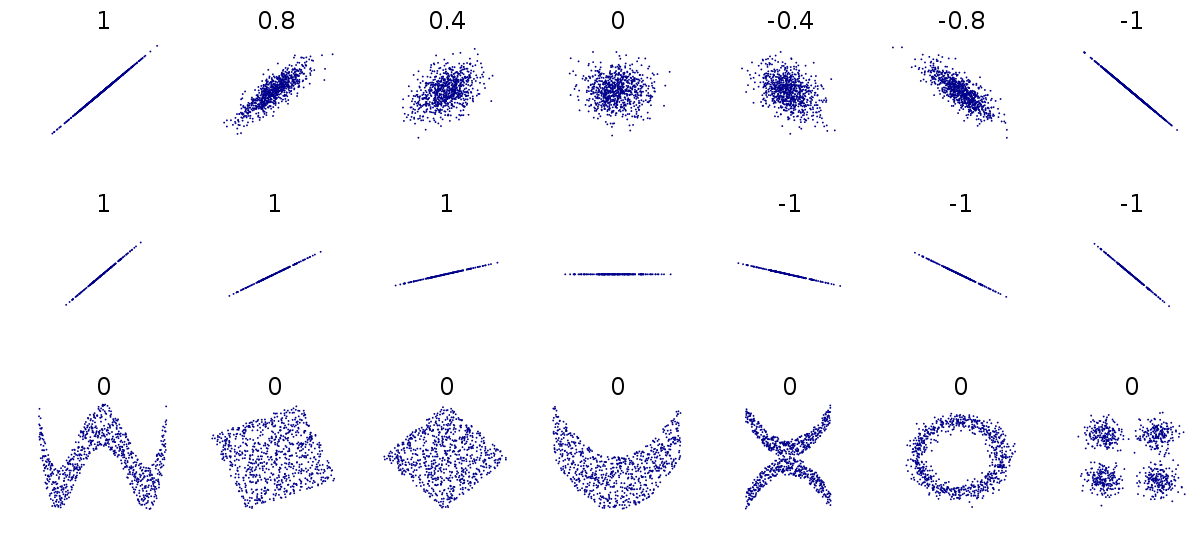
\includegraphics[scale = 0.3]{1200px-Correlation_examples2.svg.png}\\
(Taken from Wikipedia)
\end{center}
In the last example, $\text{Cov}(U,V) = \SI{-0.5}{\square\m \per \square\s}$, $\text{Var}(U) = \SI{0.5}{\square\m \per \square\s}$,\\
$\text{Var}(V) = \SI{0.6875}{\square\m \per \square\s}$, and $\rho_{uv} = \frac{0.5}{\sqrt{(0.5)(0.6875)}} \approx -0.8528$. We use the population variance and covariance for the computation, but they can be replaced by the sample counterparts at once. It may be tempting to claim that a strong negative relationship exists in this case. However, we note that the sample size here is a bit small for this result to be meaningful. Also, correlation is always dimensionless.\\
\\
We are now prepared to derive the variance formula for linear combinations of multiple variables.
\begin{proper}
\label{variancemul}
For a distribution made up of multiple variables, in the form of $Z = c_1X^{(1)} + c_2X^{(2)} + \cdots + c_nX^{(n)}$, with $\vec{c} = (c_1, c_2, \cdots, c_n)^T$ are all constants, the population variance $\text{Var}(Z)$ can be expressed as a quadratic form $\vec{c}^TQ\vec{c}$, where
\begin{align*}
Q &=
\begin{bmatrix}
\text{Cov}(X^{(1)}, X^{(1)}) & \text{Cov}(X^{(1)}, X^{(2)}) & \cdots & \text{Cov}(X^{(1)}, X^{(n)}) \\
\text{Cov}(X^{(2)}, X^{(1)}) & \text{Cov}(X^{(2)}, X^{(2)}) & \cdots & \text{Cov}(X^{(2)}, X^{(n)}) \\
\vdots & \vdots &  & \vdots \\
\text{Cov}(X^{(n)}, X^{(1)}) & \text{Cov}(X^{(n)}, X^{(2)}) & \cdots & \text{Cov}(X^{(n)}, X^{(n)}) \\
\end{bmatrix} \\
&=
\begin{bmatrix}
\text{Var}(X^{(1)}) & \text{Cov}(X^{(1)}, X^{(2)}) & \cdots & \text{Cov}(X^{(1)}, X^{(n)}) \\
\text{Cov}(X^{(2)}, X^{(1)}) & \text{Var}(X^{(2)}) & \cdots & \text{Cov}(X^{(2)}, X^{(n)}) \\
\vdots & \vdots &  & \vdots \\
\text{Cov}(X^{(n)}, X^{(1)}) & \text{Cov}(X^{(n)}, X^{(2)}) & \cdots & \text{Var}(X^{(n)}) \\
\end{bmatrix} 
\end{align*}
is the so-called covariance matrix. If $[X'] = [X'^{(1)}|X'^{(2)}|\cdots|X'^{(n)}]$ is consisted of the centered variables in columns, then $Q = \frac{1}{n}X'^TX$. To find the sample variance of $Z$, replace all $\text{Cov}(X^{(i)}, X^{(j)})$ by $q_{ij}$ in Definition \ref{covariance}.
\paragraph{Proof} To allow easier understanding, we will deal with the case of $n = 2$. However, the idea can be extended for other values of $n$. Starting from the expression in Definition \ref{variance}, we have
\begin{align*}
\text{Var}(Z) &= \frac{1}{n} \sum_{k=1}^n (z_k - \mu_z)^2 \\
&= \frac{1}{n} \sum_{k=1}^n ((c_1X^{(1)}_k + c_2X^{(2)}_k) - (c_1\mu_{x_1} + c_2\mu_{x_2}))^2 \\
&= \frac{1}{n} \sum_{k=1}^n (c_1(X^{(1)}_k - \mu_{x_1}) + c_2(X^{(2)}_k - \mu_{x_2}))^2 \\
&= \frac{1}{n} c_1^2 \sum_{k=1}^n (X^{(1)}_k - \mu_{x_1})^2 + \frac{1}{n} c_2^2 \sum_{k=1}^n (X^{(2)}_k - \mu_{x_2})^2 \\
&\quad+ \frac{2}{n} c_1c_2 \sum_{k=1}^n (X^{(1)}_k - \mu_{x_1}) (X^{(2)}_k - \mu_{x_2}) \\
&= c_1^2 \text{Cov}(X^{(1)}, X^{(1)}) + c_2^2 \text{Cov}(X^{(2)}, X^{(2)}) + 2c_1c_2 \text{Cov}(X^{(1)}, X^{(2)}) \\
&= c_1^2 \text{Cov}(X^{(1)}, X^{(1)}) + c_1c_2 \text{Cov}(X^{(1)}, X^{(2)}) \\
&\quad + c_2c_1 \text{Cov}(X^{(2)}, X^{(1)}) + c_2^2 \text{Cov}(X^{(2)}, X^{(2)}) \\
&= \sum_{i=1}^{n=2}\sum_{j=1}^{n=2} c_ic_j\text{Cov}(X^{(i)}, X^{(j)})
\end{align*}
where the terms are identified by Definition \ref{covariance}. By comparing to Definition \ref{quadform}, we realize the expression is simply
\begin{align*}
\vec{c}^TQ\vec{c} =
\begin{bmatrix}
c_1 & c_2
\end{bmatrix}
\begin{bmatrix}
\text{Cov}(X^{(1)}, X^{(1)}) & \text{Cov}(X^{(1)}, X^{(2)}) \\
\text{Cov}(X^{(2)}, X^{(1)}) & \text{Cov}(X^{(2)}, X^{(2)}) 
\end{bmatrix}
\begin{bmatrix}
c_1 \\
c_2
\end{bmatrix}
\end{align*}
for two variables situation.
\end{proper}

\begin{exmp}
From the previous wind speed example, if $W = 0.8U-0.6V$, find $\text{Var}(W)$.\\
\\
Earlier calculations show $\text{Var}(U) = \SI{0.5}{\square\m \per \square\s}$,
$\text{Var}(V) = \SI{0.6875}{\square\m \per \square\s}$, $\text{Cov}(U,V) = \text{Cov}(V,U) = \SI{-0.5}{\square\m \per \square\s}$. Plugging the values into the expression we just get, we have
\begin{align*}
\text{Var}(W) &=
\begin{bmatrix}
c_u & c_v
\end{bmatrix}
\begin{bmatrix}
\text{Var}(U) & \text{Cov}(U,V) \\
\text{Cov}(U,V) & \text{Var}(V)
\end{bmatrix}
\begin{bmatrix}
c_u \\
c_v
\end{bmatrix} \\
&=
\begin{bmatrix}
0.8 & -0.6
\end{bmatrix}
\begin{bmatrix}
0.5 & -0.5 \\
-0.5 & 0.6875
\end{bmatrix}
\begin{bmatrix}
0.8 \\
-0.6
\end{bmatrix} \\
&= \SI{1.0475}{\square\m \per \square\s}
\end{align*}
\end{exmp}

\subsection{Principal Component Analysis}
A common practice in Earth Science is to reduce the dimensions of a large set of data. Given a large number of variables, each with a substantial amount of measurements, we want to process them to extract and retain the most important features or signals. Principal Component Analysis, which also known as Empirical Orthogonal Function in atmospheric science, is the mainstream method to achieve this goal, by finding the pattern which maximizes the variance of the dataset. It will be explained slowly with some diagrams and helper theorems.\\
\\
Consider the simplest case with two variables, or time-series $X$ and $Y$ first. Assume they have $n$ pairs of entries, from $\vec{x_1}^T = (x_1, y_1)^T$ to $\vec{x_n}^T = (x_{n}, y_{n})^T$. We can compute the covariance matrix $Q$, introduced in the last section. Principal Component Analysis want to find a unit vector $\textbf{e}$, so that the variance of data along the direction indicated by $\textbf{e}$, which is $\textbf{e}^T Q \textbf{e}$ following from Properties \ref{variancemul}, is maximized.
\begin{center}
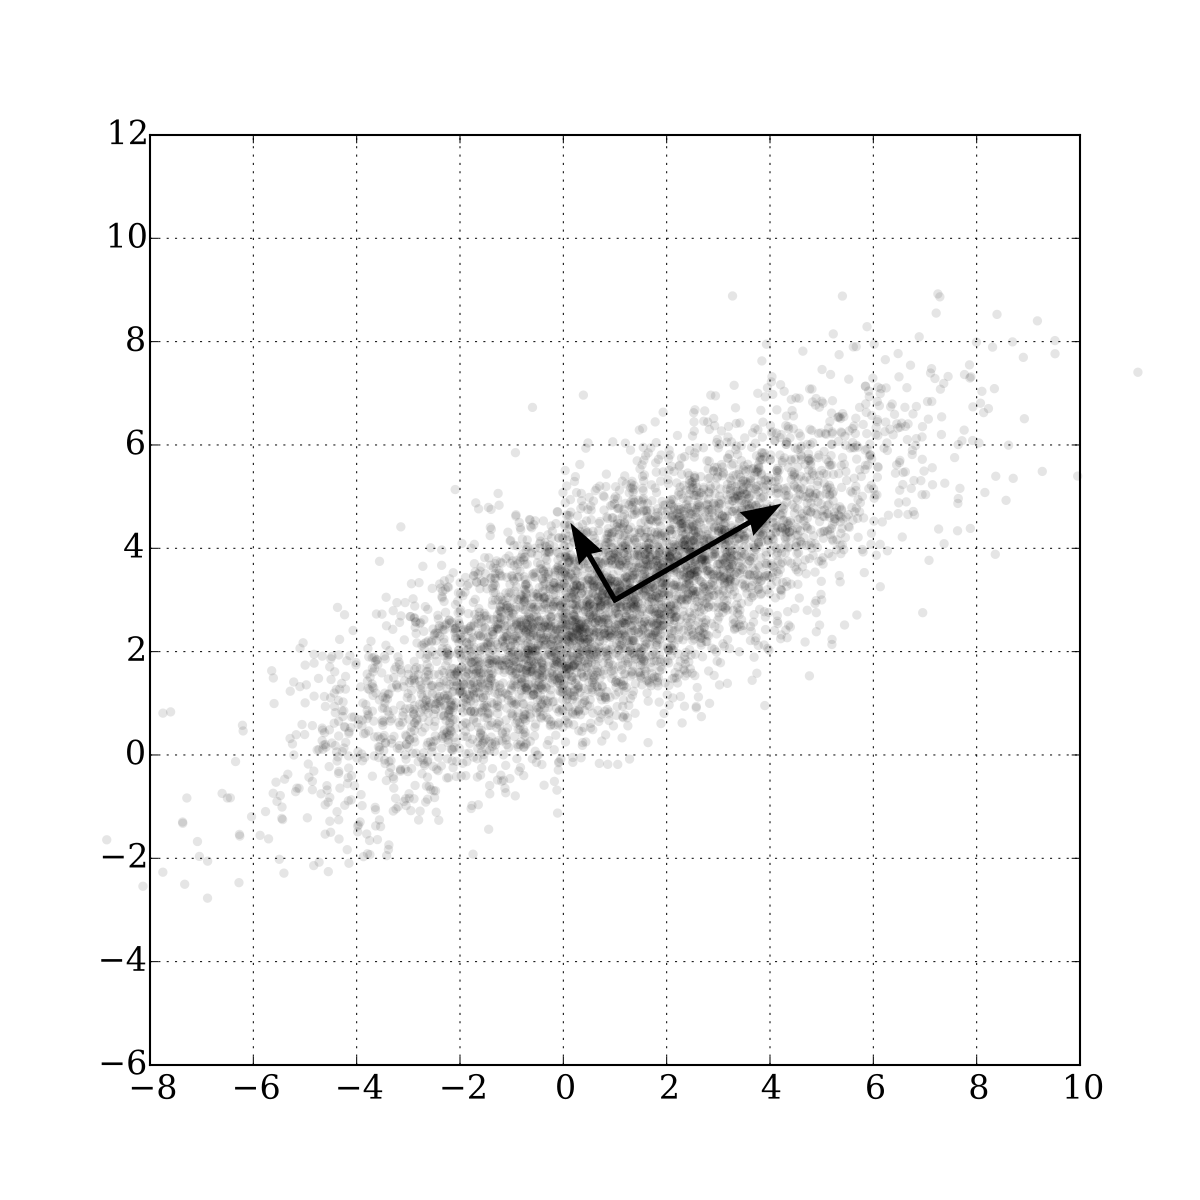
\includegraphics[scale = 0.15]{1200px-GaussianScatterPCA.svg.png}\\
Two principal axes found by Principal Component Analysis for a set of data. The longer vector represents the direction of largest variance. The data points can be seen to spread more along that direction. (Taken from Wikipedia)
\end{center}
Now the problem is to find, under what situation $\textbf{e}^T Q \textbf{e}$ will assume its largest value. Here, we introduce a famous technique, called the Lagrange Multiplier, which requires some knowledge in Calculus. As before, we will proceed with the 2 variables case for brevity.
\begin{thm}
\label{LagrangeMul}
To find the extremal values attained by a function $f(u,v,\cdots)$, under the constraint $g(u,v,\cdots) = 0$, we consider the expression
\begin{align*}
h(u,v,\cdots) = f(u,v,\cdots) - \lambda g(u,v,\cdots)
\end{align*}
where $\lambda$ is a constant to be determined by solving the system
\begin{align*}
\begin{cases}
\partial h/\partial u &= 0 \\
\partial h/\partial v &= 0 \\
\cdots &= 0
\end{cases}
\end{align*}
$\partial/\partial u$ and $\partial/\partial v$ means differentiating with $u$ and $v$ only while treating other variables as constants. The values of $u$ and $v$ to reach the extremums are also inferred from the set of equations above. 
\end{thm}
We are now going to find the value of $x'$ and $y'$ so that $\textbf{e}^T Q \textbf{e}$ obtains the maximum for $\textbf{e}^T = (x',y')$. The constraint is that $\textbf{e}$ is a unit vector as a direction, and hence by the method of Lagrange Multiplier outlined in Theorem \ref{LagrangeMul}, we have
\begin{align*}
g(x',y') = x'^2 + y'^2 - 1 = 0
\end{align*}
and with $f(x',y') = \textbf{e}^T Q \textbf{e}$
\begin{align*}
h(x',y') &= (\textbf{e}^T Q \textbf{e}) - \lambda(x'^2 + y'^2 - 1) \\
&= x'^2 \text{Cov}(X, X) + 2x'y' \text{Cov}(X, Y) + y'^2\text{Cov}(Y, Y) - \lambda(x'^2 + y'^2 - 1)
\end{align*}
according to Properties \ref{variancemul}. Carrying out the differentiation gives
\begin{align*}
\begin{cases}
\partial h/\partial x' &= 2x'\text{Cov}(X, X) + 2y'\text{Cov}(X, Y) - 2\lambda x' = 0 \\
\partial h/\partial y' &= 2x'\text{Cov}(X, Y) + 2y'\text{Cov}(Y, Y) - 2\lambda y' = 0
\end{cases}    
\end{align*}
This system can be immediately be recognised as
\begin{align*}
\begin{bmatrix}
\text{Cov}(X, X)-\lambda & \text{Cov}(X, Y) \\
\text{Cov}(Y, X) & \text{Cov}(Y, Y)-\lambda
\end{bmatrix}
\begin{bmatrix}
x' \\
y'
\end{bmatrix} &= 0\\
(Q-\lambda I)\vec{x'} &= 0
\end{align*}
which is an eigenvalue problem like those in Section \ref{eigensection}. Hence we conclude that $f(x',y') = \textbf{e}^T Q \textbf{e}$ attains its extremal values when $\textbf{e}^T = (x',y')^T$ is the unit eigenvector of $Q$. The corresponding magnitude of variance ${\textbf{e}^{(j)}}^T Q \textbf{e}^{(j)}$ for the $j$-th eigenvector is
\begin{align*}
{\textbf{e}^{(j)}}^T (Q \textbf{e}^{(j)}) &= {\textbf{e}^{(j)}}^T (\lambda^{(j)} \textbf{e}^{(j)}) \\
&= \lambda^{(j)} ({\textbf{e}^{(j)}}^T \textbf{e}^{(j)}) \\
&= \lambda^{(j)} (\hat{e}^{(j)} \cdot \hat{e}^{(j)}) \\
&= \lambda^{(j)} \norm{\hat{e}^{(j)}} \\
&= \lambda^{(j)}
\end{align*}
where we have used the facts that $Q \textbf{e}^{(j)} = \lambda^{(j)} \textbf{e}^{(j)}$ as per Definition \ref{eigen} and the length of a unit vector is $1$. This means that the variance along the direction of eigenvector is exactly the corresponding eigenvalue. To generalize for more variables, we have the following results.
\begin{thm}
For a covariance matrix $Q$ which happens to be symmetric, the variance $\textbf{e}^T Q \textbf{e}$ achieves its maximum value $\lambda_1$ along the direction $\textbf{e}^{(1)}$, which are the largest eigenvalue of $Q$ and the associated unit eigenvector. \\
Generally, if $Q$ has the orthonormal eigenvectors $\textbf{e}^{(1)}, \textbf{e}^{(2)}, \cdots, \textbf{e}^{(n)}$, arranged by the eigenvalues $\lambda_1 > \lambda_2 > \cdots > \lambda_n$, then the largest variance will be $\lambda_1$ when the direction is along $\textbf{e}^{(1)}$, the second largest will be  $\lambda_2$ for $\textbf{e}^{(2)}$ and so on, with the smallest variance being $\lambda_n$ for $\textbf{e}^{(n)}$. This set of linearly independent eigenvectors are called the Principal Directions in Principal Component Analysis.
\end{thm}
As a side note, any quadratic form $\hat{x}^TA\hat{x}$ will attain its maximum and minimum when $\hat{x}$ is the eigenvector that represents the largest and smallest eigenvalue, which are also the value $\hat{x}^TA\hat{x}$ takes when it happens. This is under the constraint that $\hat{x}$ is a unit vector, and has the name Constrained Extremum Theorem.\\
\\
Going back to the problem of Principal Component Analysis, for each Principal Directions $\textbf{e}^{(j)}$ and the variance $\lambda_{j}$, we can compute the ratio of explained variance, which is the fraction $\lambda_{j}$ over the total variance, that is the sum of eigenvalues for the covariance matrix. This number allows us to access how well the Principal Direction contributes to the total variance.\\
\\
With the set of orthonormal principal directions at hand, we can treat them as a coordinate basis and subsequently perform a rotation on the data as we have done earlier. Constructing a transition matrix made up of the Principal Directions $[\textbf{e}] = [\textbf{e}^{(1)}|\textbf{e}^{(2)}|\cdots|\textbf{e}^{(n)}]$, the new coordinates are $\vec{u} = [\textbf{e}]^T \vec{x}$ as suggested by Section \ref{orthogeometricsub}. $\vec{u_i}$ can be regarded to be the projection of $\vec{x_i}^T = (x_i, y_i)^T$ the $i$-th pair of data onto the principal directions and is called the Principal Components. By doing an orthogonal rotation on $Q$ by $[\textbf{e}]$, the resulted quantities $[\textbf{e}]^T Q[\textbf{e}]$ will be a diagonal matrix with non-trivial elements being the variances along the Principal Directions. \\
\\
Usually, at the start we will detrend the data and remove the mean from each variable, such that we use $x'_i = x_i - \bar{x}$ and $y'_i = y_i - \bar{y}$ to replace $x_i$ and $y_i$.

\begin{exmp}
The temperature data of two cities $M$ and $N$ are as follows.
\begin{center}
\begin{tabular}{|c|c|c|}
\hline
(in \si{\degree C}) & $M$ & $N$\\
\hline
1st Day & 22.1 & 22.3 \\
\hline
2nd Day & 21.8 & 21.6 \\
\hline
3nd Day & 20.9 & 21.2 \\
\hline
4th Day & 21.6 & 21.7 \\
\hline
5th Day & 23.4 & 23.2 \\
\hline 
6th Day & 24.7 & 24.1 \\
\hline 
7th Day & 22.0 & 23.9 \\
\hline 
8th Day & 22.1 & 22.4 \\
\hline 
\end{tabular}
\end{center}
Perform Principal Component Analysis and find the strongest Principal Direction, and extract the time-series related to this mode.\\
\\
After detrending, the data are
\begin{center}
\begin{tabular}{|c|c|c|}
\hline
(in \si{\degree C}) & $M'$ & $N'$\\
\hline
1st Day & -0.225 & -0.25 \\
\hline
2nd Day & -0.525 & -0.95 \\
\hline
3nd Day & -1.425 & -1.35 \\
\hline
4th Day & -0.725 & -0.85 \\
\hline
5th Day & 1.075 & 0.65 \\
\hline 
6th Day & 2.375 & 1.55 \\
\hline 
7th Day & -0.325 & 1.35 \\
\hline 
8th Day & -0.225 & -0.15 \\
\hline 
\end{tabular}
\end{center}
From Properties \ref{variancemul}, the sample covariance matrix is
\begin{align*}
Q = 
\frac{1}{8-1}
\begin{bmatrix}
\vec{m'}\cdot\vec{m'} & \vec{m'}\cdot\vec{n'} \\
\vec{n'}\cdot\vec{m'} & \vec{n'}\cdot\vec{n'} 
\end{bmatrix} =
\begin{bmatrix}
1.405 & 1.01 \\
1.01 & 1.1686
\end{bmatrix}
\end{align*}
The unit eigenvectors for $Q$ and thus the Principal Directions can be found to be $\textbf{e}^{(1)} = (0.747, -0.665)^T$ of larger variance $\lambda_1 = \SI{2.304}{\square {(\degree C)}}$, and $\textbf{e}^{(2)} = (0.665, 0.747)^T$ of smaller variance $\lambda_2 = \SI{0.270}{\square {(\degree C)}}$. The first principal component accounts for $2.304 / (2.304+0.270) \approx 89.5\%$ of the total variance.\\
\\
We can project every pair of data $\vec{x'}_i^T = (m'_i, n'_i)^T$ onto the principal directions by computing $\vec{u}_i = [\textbf{e}]^T\vec{x'}_i$, where $[\textbf{e}] = [\textbf{e}^{(1)}|\textbf{e}^{(2)}]$. The principal values are 
\begin{center}
\begin{tabular}{|c|c|c|c|c|c|c|c|c|}
\hline
(in \si{\degree C}) & D-1 & D-2 & D-3 & D-4 & D-5 & D-6 & D-7 & D-8 \\
\hline
$u^{(1)}$ & -0.334 & -1.024 & -1.962 & -1.107 & 1.235 & 2.805 & 0.655 & -0.268 \\
\hline
$u^{(2)}$ & -0.037 & -0.361 & -0.061 & -0.153 & -0.229 & -0.421 & 1.225 & 0.038 \\
\hline
\end{tabular}
\end{center}
In details, the principal components for the first day is computed by
\begin{align*}
\begin{bmatrix}
u_1^{(1)} \\
u_1^{(2)} 
\end{bmatrix}
=
\begin{bmatrix}
0.747 & 0.665 \\
-0.665 & 0.747
\end{bmatrix}
\begin{bmatrix}
-0.225 \\
-0.25
\end{bmatrix}
\end{align*}
The original dataset can be recovered by $\vec{x'}_i = [\textbf{e}]\vec{u'}_i$. If we want to extract the signals originated from the first Principal Directions, we can simply remove other column eigenvectors in $[\textbf{e}]$ and discard other principal values in $\vec{u'}_i$. The time-series reconstructed by the first mode is hence computed by $x'_i = \textbf{e}^{(1)}u_i^{(1)}$, which are
\begin{center}
\begin{tabular}{|c|c|c|c|c|c|c|c|c|}
\hline
(in \si{\degree C}) & D-1 & D-2 & D-3 & D-4 & D-5 & D-6 & D-7 & D-8 \\
\hline
$M'$ & -0.250 & -0.765 & -1.466 & -0.827 & 0.923 & 2.095 & 0.489 & -0.200 \\
\hline
$N'$ & -0.222 & -0.681 & -1.304 & -0.736 & 0.821 & 1.864 & 0.435 & -0.178 \\
\hline
\end{tabular}
\end{center}
\end{exmp}
\newpage
\begin{center}
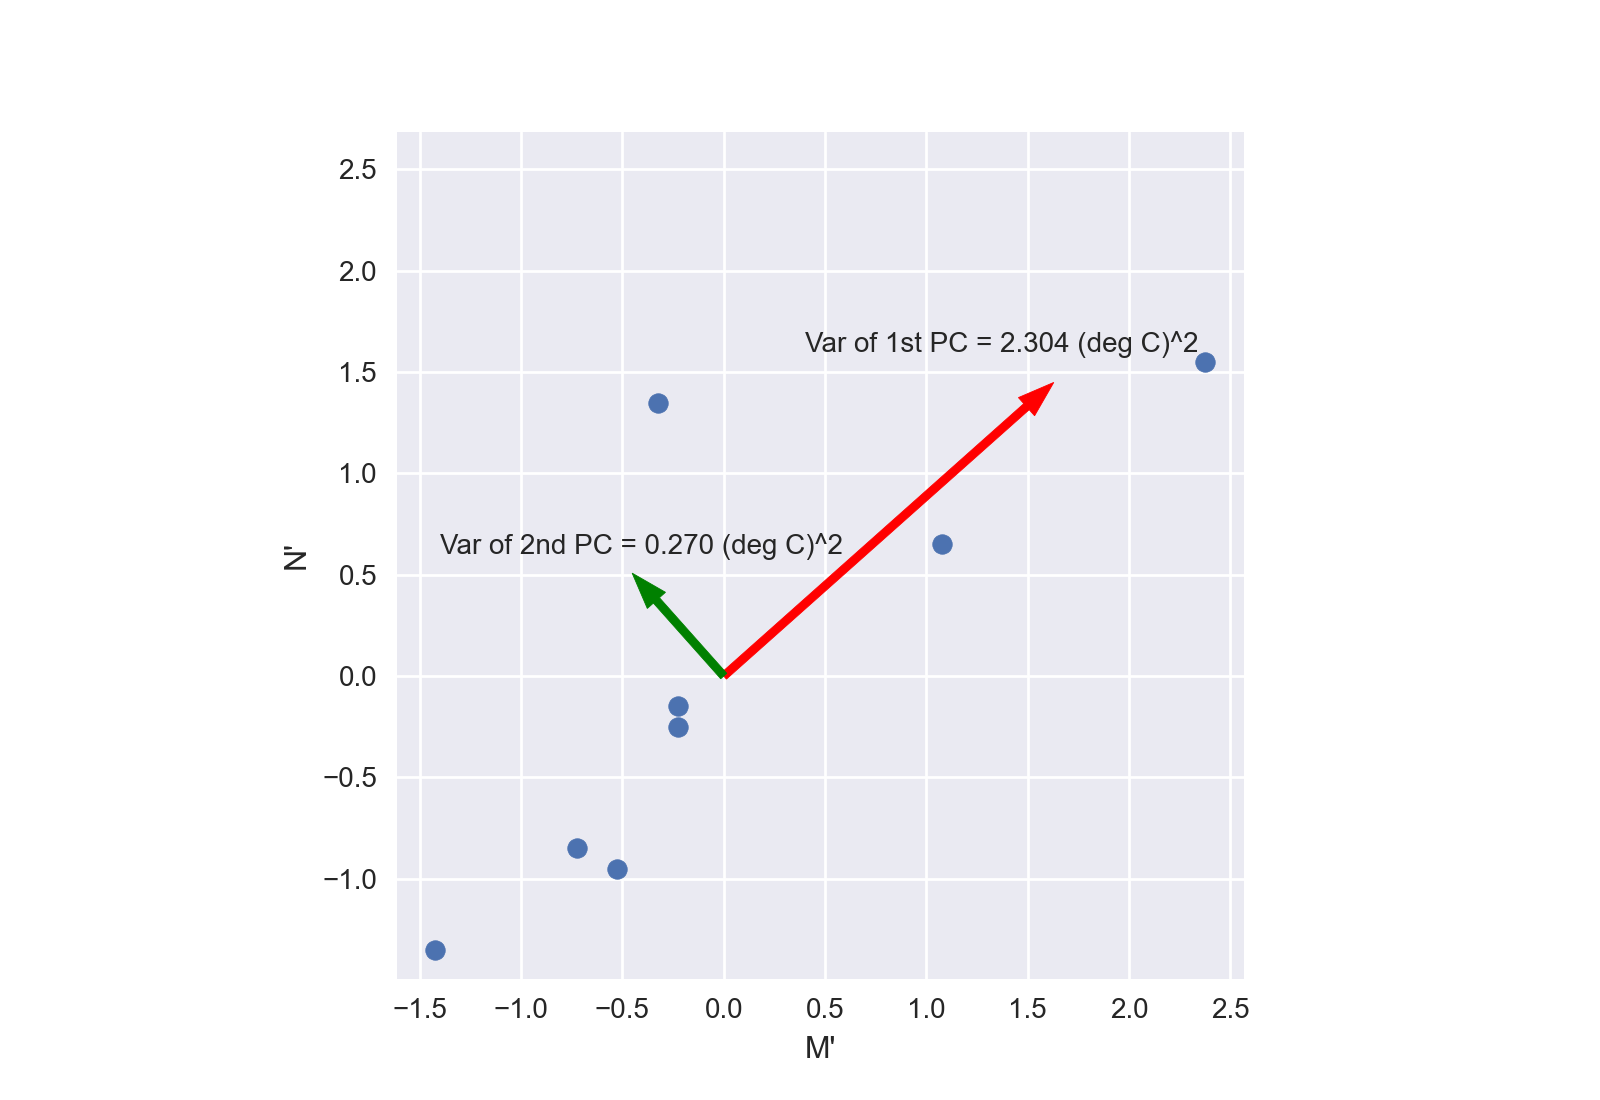
\includegraphics[scale = 0.6]{LAEOF.png}\\
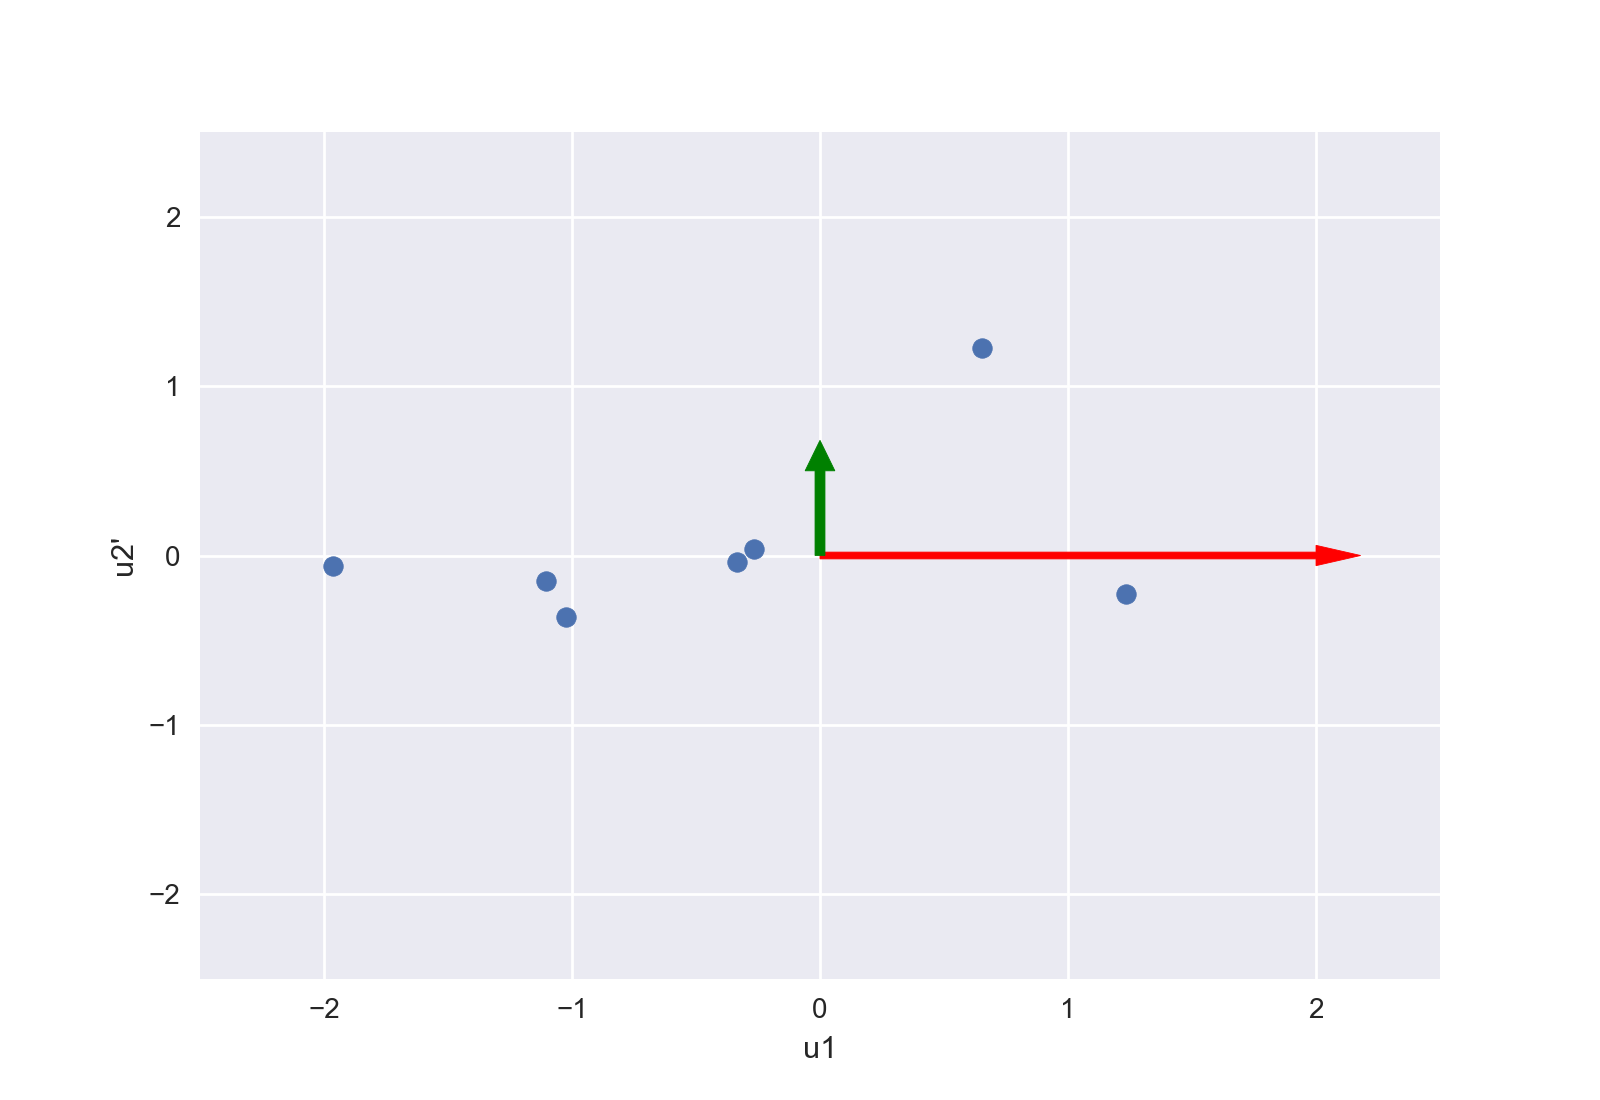
\includegraphics[scale = 0.6]{LAEOF2.png}\\
The data before and after rotation by the principal directions, with the one with larger/smaller variance shown as red/green.
\end{center}
\begin{center}
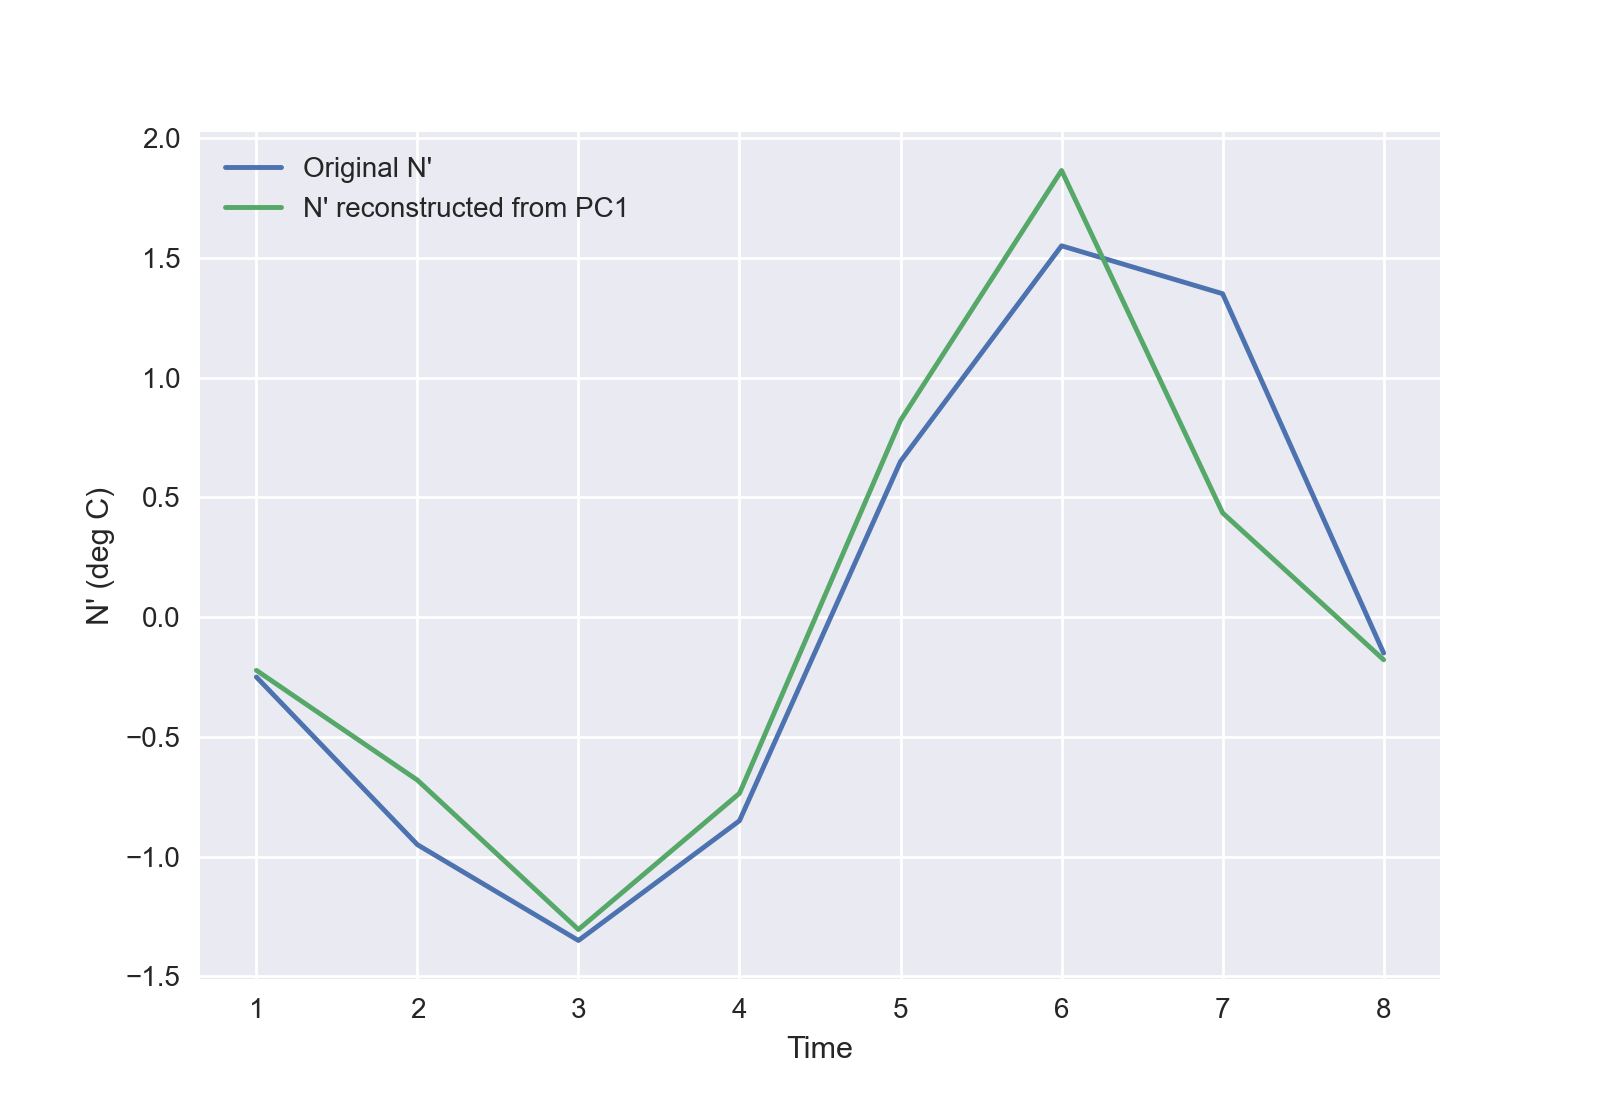
\includegraphics[scale = 0.6]{LAEOF3.png}\\
Comparison between the original anomaly and the first mode for $N'$.
\end{center}

\section{Exercise}

\begin{Exercise}
Identify the following conic sections and eliminate the cross-product terms by an appropriate rotation.
\begin{enumerate}[label=(\alph*)]
\item $x^2 + 5xy + 3y^2 = 1$,
\item $x^2 - xy + 2y^2 = 4$,
\item $x^2 + 2xy + y^2 = 1$, what is the curve generated? 
\end{enumerate}
\end{Exercise}

\begin{Exercise}
Find a new expression for the standard hyperbola $y^2 - x^2 = 1$ if a anti-clockwise rotation of $75$ degrees is done. What about a reflection along the $x$-axis?
\end{Exercise}

\begin{Exercise}
Three-dimensional quadrics can also be treated in a similar fashion to two-dimensional conic sections. Find the length of three axes for an ellipsoid $x^2 + y^2 + z^2 + 0.5xy - yz + 0.5xz = 1$ by doing an orthogonal coordinate transformation. What is the requirement for a three-dimensional quadratic form to represent an ellipsoid?
\end{Exercise}

\begin{Exercise}
Find the covariance matrix for three pressure time-series over $10$ days at cities $X$, $Y$, $Z$ (in hPa, relative to $1000$ hPa), which take the values
\begin{center}
\begin{tabular}{|c|c|c|}
\hline
$X$ & $Y$ & $Z$ \\
\hline
17 & 19 & 22 \\
\hline
18 & 16 & 25 \\
\hline
14 & 15 & 17 \\
\hline
19 & 21 & 23 \\
\hline
24 & 22 & 26 \\
\hline
21 & 20 & 23 \\
\hline 
28 & 26 & 29 \\
\hline
24 & 25 & 22 \\
\hline
20 & 21 & 27 \\
\hline
23 & 22 & 24 \\
\hline
\end{tabular}
\end{center}
Find the variance of $W = X - 0.5Y - 0.5Z$.
\end{Exercise}

\begin{Exercise}
Carry out Principal Component Analysis on the data set above. Find the Principal Directions and the ratio of explained variance for each of them. Reconstruct the data using the first Principal Direction with largest variance only.
\end{Exercise}

